\chapter{Appendices}
\label{ch:appendices}

The printed appendices for this thesis are intentionally minimal.
All the data I used are included in the electronic appendices,
along with the custom-written analysis and plotting code.
Any interested reader who has not received the DVD with this material is
invited to contact me at \texttt{zac.hatfield.dodds@gmail.com} for a copy.


\section*{Additional Figures}
This section contains figures which would unnecessarily disrupt the
flow of the thesis, but are directly referenced in the text and therefore
should not be left to the electronic appendices.


\begin{figure}[p]
    \centering
    \frame{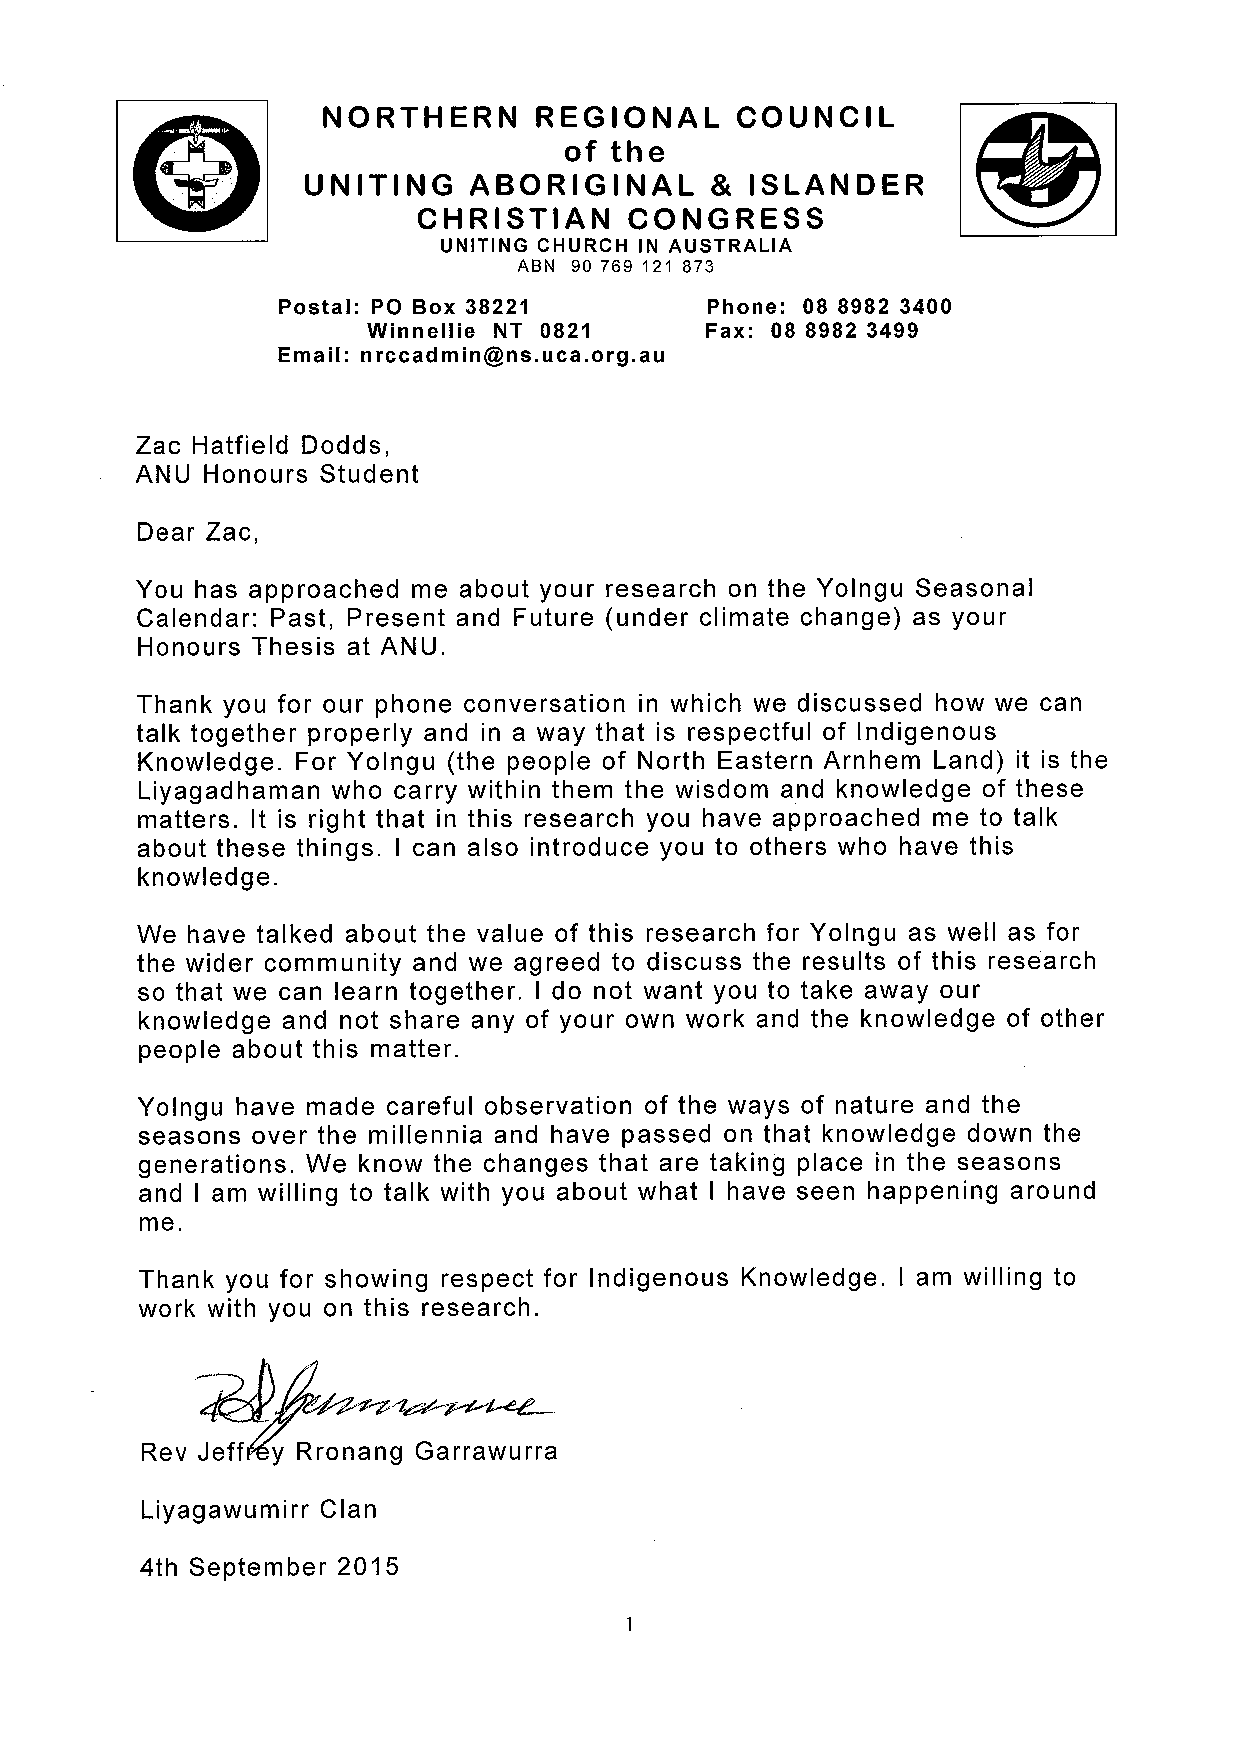
\includegraphics[width=0.9\textwidth]{invitation-letter.pdf}}
    \caption[Letter of invitation for collaborative research]{
        The formal invitation to study Yolngu seasons,
        and share results with both first and second peoples.
        Pre-existing relationships, with Yolngu and non-indigenous people,
        were essential in arranging this collaboration.
        }
    \label{app:invitation-letter}
\end{figure}

\begin{figure}[p]
    \centering
    \includegraphics[width=\textwidth]{galiwinku/seabreeze-direction.pdf}
    \caption[3-hourly wind direction heatmaps, Galiwinku]{
        3-hourly wind direction heatmaps for Galiwinku,
        showing the northerly sea-breeze in the afternoon.
        Based on this figure, I judged that the difference between
        3pm and 6pm wind for season detection is small enough that
        I prefer the meteorological standard (3pm) over Yolngu advice (6pm).}
    \label{fig:galiwinku-seabreeze-direction}
\end{figure}
